% Standalone source. Compile with pdflatex or latexmk -pdf.
\documentclass[11pt]{article}
\usepackage[T1]{fontenc}
\usepackage{lmodern}
\usepackage[margin=1in]{geometry}
\usepackage{amsmath,amssymb,amsthm,mathtools}
\usepackage{microtype,enumitem,booktabs,longtable,array,xcolor,listings}
\usepackage{tikz}
\usetikzlibrary{arrows.meta,positioning}
\usepackage{xurl}
\usepackage[colorlinks=true,linkcolor=blue!45!black,urlcolor=blue!45!black]{hyperref}
\usepackage{fancyhdr}
\pagestyle{fancy}\fancyhf{}
\fancyhead[L]{\small Hyperplane cohomology: Lean blueprint}
\fancyhead[R]{\small\thepage}
\setlength{\headheight}{14pt}
\setlength{\emergencystretch}{2em}
\setlist{itemsep=3pt,topsep=5pt}
\lstset{basicstyle=\ttfamily\footnotesize,breaklines=true,columns=fullflexible,keepspaces=true,frame=single,rulecolor=\color{black!20},xleftmargin=4pt,xrightmargin=4pt}
\newcommand{\A}{\mathbb A}
\newcommand{\PP}{\mathbb P}
\newcommand{\Gm}{{\mathbb G_m}}
\newcommand{\Z}{\mathbb Z}
\newcommand{\N}{\mathbb N}
\newcommand{\cA}{\mathcal A}
\newcommand{\cP}{\mathcal P}
\newcommand{\OS}{\operatorname{OS}}
\newcommand{\pOS}{\overline{\operatorname{OS}}}
\newcommand{\im}{\operatorname{im}}
\newcommand{\kerop}{\operatorname{ker}}
\newcommand{\res}{\operatorname{res}}
\newcommand{\codim}{\operatorname{codim}}
\newcommand{\Hom}{\operatorname{Hom}}
\newcommand{\Spec}{\operatorname{Spec}}
\newcommand{\SH}{\operatorname{SH}}
\newcommand{\one}{\mathbf 1}
\newcommand{\logc}[1]{[#1]}
\newcommand{\planned}[1]{\texttt{\detokenize{#1}}}
\newtheorem{theorem}{Theorem}[section]
\newtheorem{lemma}[theorem]{Lemma}
\newtheorem{proposition}[theorem]{Proposition}
\newtheorem{corollary}[theorem]{Corollary}
\theoremstyle{definition}
\newtheorem{definition}[theorem]{Definition}
\theoremstyle{remark}
\newtheorem{remark}[theorem]{Remark}

\newcommand{\lean}[1]{\par\smallskip{\footnotesize\color{blue!50!black}\textsf{Planned declaration: }\nolinkurl{#1}}\par\smallskip}
\newcommand{\uses}[1]{}
\hypersetup{pdftitle={Hyperplane arrangement cohomology: a Lean formalization blueprint},pdfauthor={Prepared for Adam Topaz}}
\title{Hyperplane arrangement cohomology\\\large A Lean formalization blueprint from standard cohomology axioms}
\author{Prepared for Adam Topaz}
\date{6 November 2026}
\begin{document}
\maketitle
\begin{abstract}
The target is a formal proof of the Orlik--Solomon structure theorem for any ordinary cohomology theory with products, a dimension axiom at the point, affine-line invariance, and compatible localization and divisor purity. We specify the interfaces, geometric constructions, intermediate statements, and proof dependencies needed for an implementation in Lean. Tate twists remain explicit, coefficients need not be a field, and the base field is arbitrary. The projective theorem is included. A separate abstract stable-category extension covers generalized cohomology groups.

This is a proof blueprint, not a completed Lean development. Every Lean name below is proposed. The displayed signatures are design sketches and have not been elaborated. No theorem is marked as formally verified. The accompanying source contains dependency annotations and an independently checked dependency manifest.
\end{abstract}
\clearpage
\tableofcontents
\newpage
\section{The formal target and the trust boundary}

Fix a field $k$ and a commutative coefficient ring $R$. A split arrangement is a finite set of distinct hyperplanes defined over $k$. The affine complement is $U_{\cA}=\A^n_k\setminus\bigcup\cA$. For a nonempty projective arrangement $\cP$ in $\PP^n_k$, write $U_{\cP}$ for its complement and $c\cP$ for its central cone arrangement.

The principal public theorem should construct canonical graded algebra isomorphisms
\[
 \OS_R(\cA)\simeq\bigoplus_{q\geq0}H^{q,q}(U_{\cA}),\qquad
 \pOS_R(\cP)\simeq\bigoplus_{q\geq0}H^{q,q}(U_{\cP}),
\]
where $H^{p,w}$ means cohomological degree $p$ and Tate twist $w$. Affine generators map to $\logc{f_H}$; projective differences map to $\logc{\ell_i/\ell_j}$. The construction must be independent of scaling the equations and, in the projective case, of the hyperplane chosen at infinity.

For implementation we prove a stronger total-ring statement first. Put
\[
 B=\bigoplus_{w\in\Z}H^{0,w}(k),\qquad
 C(X)=\bigoplus_{(p,w)\in\Z^2}H^{p,w}(X).
\]
The target is a bigrading-preserving $B$-algebra equivalence
\[
 \Phi_{\cA}:\OS_B(\cA)\simeq_B C(U_{\cA}).
\]
Here a generator has bidegree $(1,1)$, while $B_w$ has bidegree $(0,w)$. It follows that
\[
 H^{p,w}(U_{\cA})\simeq_R
 \OS_R^p(\cA)\otimes_R B_{w-p}\quad(p\geq0),
\]
and $H^{p,w}=0$ for $p<0$ or $p>n$. Taking $B_0\simeq R$ gives the diagonal theorem. For genuine Tate lines this is the usual formula $H^p(U)\simeq\OS_R^p(\cA)(-p)$. We never choose a generator of every Tate line.

\paragraph{What is conditional, and what is proved?}
The cohomology theory is a structure supplied to the theorem. Its fields express standard axioms. The geometry interface is a separate structure supplying actual objects and commutative diagrams; its implementation uses affine linear algebra and localization. The structure theorem is proved from these two interfaces. To obtain an unconditional theorem about a named realization, one must additionally construct its cohomology instance. This blueprint does not pretend that Lean already contains \(\ell\)-adic or rigid cohomology with all required properties.

No cohomology field may assert logarithmic generation, arrangement vanishing, surjectivity of residues, vanishing of Gysin maps, a short exact deletion sequence, freeness, or the desired algebra equivalence. These are outputs of the proof. Do not use global \planned{axiom} declarations. Quantify the public results over structures with proof fields, and eventually audit the results with \planned{\#print axioms}. The usual foundational axioms used by mathlib are compatible with the project; \planned{sorryAx} is not.

\paragraph{The coefficient boundary.}
The ordinary theorem assumes the point has cohomology only in cohomological degree zero. Arithmetic cohomology over a nonclosed field usually fails this axiom. So do many generalized theories. Their additive calculation is handled separately in Section~\ref{sec:stable}; the classical exterior ring presentation is not imposed on them.

\section{Representations and reusable algebra}

\begin{definition}[Internal bigrading]\label{def:grading}
\lean{ArrangementCohomology.Grading.InternalBigrading}
An internal bigrading of an $R$-algebra $T$ consists of $R$-submodules $T_{p,w}\subseteq T$, a direct-sum decomposition
\[
 \bigoplus_{(p,w)\in\Z^2} T_{p,w}\simeq_R T,
\]
and proofs that $1\in T_{0,0}$ and $T_{p,w}T_{q,v}\subseteq T_{p+q,w+v}$. The equivalence is induced by the inclusions, not an unrelated module equivalence. A homogeneous map of shift $(a,b)$ sends $T_{p,w}$ into $T'_{p+a,w+b}$.
\end{definition}

Use mathlib's internal direct-sum machinery or wrap it behind this interface. The grading pieces are \emph{$R$-submodules}, not $B$-submodules: multiplying by $B_v$ changes the weight. The total ring can nevertheless be a $B$-algebra. Direct sums have finite support; a product over all degrees would change the mathematical object.

The sign in graded commutativity depends only on the first degree. Define $\epsilon(p)=1$ if $p\in\Z$ is even and $-1$ otherwise, with values in $R$. Prove $\epsilon(p+q)=\epsilon(p)\epsilon(q)$ and use $\epsilon(pq)$ in $xy=\epsilon(pq)yx$. This avoids ambiguous exponentiation by negative integers. No assumption that $2$ is invertible is permitted.

\begin{lemma}[Homogeneous extraction]\label{lem:extraction}
\lean{ArrangementCohomology.Grading.homogeneous_preimage}
\uses{def:grading}
For a homogeneous linear map of a fixed degree shift, a homogeneous element in its range has a homogeneous preimage of the corresponding degree. A bijective homogeneous map has a homogeneous inverse. For composable homogeneous maps, exactness of the total maps is equivalent to exactness in every appropriately shifted homogeneous component.
\end{lemma}
\begin{proof}
Decompose a preimage into its finitely many homogeneous components and project the equality to the required degree. The shift is a translation of $\Z^2$, hence injective, so only one component contributes. For exactness, first use total exactness and then this extraction; the converse follows by lifting each of finitely many homogeneous components and summing. Record the shifts explicitly in the statement of the componentwise equivalence.
\end{proof}

\begin{definition}[A quotient usable by both algebra and linear maps]\label{def:twosided}
\lean{ArrangementCohomology.Algebra.RelationQuotient}
For a possibly noncommutative $B$-algebra $T$ and a set $\mathcal R\subseteq T$, let
\[
 J(\mathcal R)=\operatorname{span}_B\{a r b:a,b\in T,\ r\in\mathcal R\}.
\]
The relation quotient is $T/J(\mathcal R)$, with its ring and $B$-algebra structure. The quotient's underlying module is the indicated submodule quotient.
\end{definition}

\begin{lemma}[Quotient API]\label{lem:quotient-api}
\lean{ArrangementCohomology.Algebra.RelationQuotient.universalProperties}
\uses{def:twosided}
The submodule $J(\mathcal R)$ is stable under left and right multiplication. Algebra maps out of the quotient correspond to algebra maps killing every relator. Linear maps out of the quotient correspond to linear maps killing $J(\mathcal R)$; it suffices to kill every $arb$. If the relators are homogeneous in an internally graded algebra, the quotient has the induced internal grading.
\end{lemma}
\begin{proof}
Prove multiplicative stability by submodule-span induction. Then $x\sim y$ iff $x-y\in J$ is a ring congruence. Its quotient is canonically the module quotient, and multiplication is well defined because changing either input changes the product by an element of $J$. The two universal properties follow from their respective quotient lifts. For the grading, decompose $a$ and $b$: every homogeneous component of $arb$ is a sum of contexts of homogeneous relators, hence lies in $J$. The direct decomposition therefore descends.
\end{proof}

This small API avoids committing the rest of the proof to a particular quotient implementation. Mathlib has \planned{RingQuot} and \planned{RingQuot.liftAlgHom}, which handle noncommutative algebras. They can be used internally, provided the equivalence with the module quotient and the linear descent lemma are proved. Alternatively use a two-sided ideal or ring congruence directly. An algebra universal property alone is insufficient for the deletion argument below.

\begin{lemma}[Exterior words]\label{lem:exterior-words}
\lean{ArrangementCohomology.Algebra.exteriorWordLemmas}
Let $I$ be a finite type and $E=\bigwedge_B(B^{(I)})$, implemented using \planned{ExteriorAlgebra B (I →₀ B)}. Ordered words in its standard generators span $E$. Repeated letters give zero; permutation of a word multiplies it by the permutation sign; any two words supercommute according to their lengths. For square-zero, pairwise anticommuting elements $x_i$ of a $B$-algebra, the linear map $B^{(I)}\to T$ sending the basis to $x_i$ takes \emph{every} vector to a square-zero element and hence extends uniquely to $E\to_B T$.
\end{lemma}
\begin{proof}
Use the tensor/exterior algebra induction principle for spanning. Derive anticommutation from $(v+w)^2=v^2=w^2=0$, and move letters successively to prove the word statements. For the last assertion, expand the square of a finite sum. Diagonal terms vanish and off-diagonal pairs cancel. This proof works in characteristic two and with $2$-torsion. It supplies exactly the condition required by \planned{ExteriorAlgebra.lift}; checking only the basis vectors is not its full input.
\end{proof}

\section{The geometry layer}

\begin{definition}[Affine arrangements]\label{def:arrangement}
\lean{ArrangementCohomology.Geometry.AffineArrangement}
An affine hyperplane in a finite-dimensional $k$-vector space $V$ is a nonempty proper affine subspace of codimension one. An arrangement is a finite set of such hyperplanes. An equation for $H$ is an affine map $f_H:V\to k$ with nonzero linear part and zero locus $H$.
\end{definition}

Use \planned{Finset} for the support, and its subtype as the finite generator type. Classical decidable equality is harmless. Use \planned{List} for signed words and boundary sums; an unordered finite set is not enough to specify their signs. One may first implement $V=k^n$, but the induction statements must quantify over all dimensions. An affine-subspace representation makes the geometric intersection lemmas clearer than quotienting equations at the outset.

\begin{lemma}[Equations and affine intersections]\label{lem:equations}
\lean{ArrangementCohomology.Geometry.equationLemmas}
\uses{def:arrangement}
Every hyperplane has an equation. Two equations for the same hyperplane differ by a unique scalar in $k^\times$. A nonempty intersection of hyperplanes has a $k$-point and is an affine space with direction the intersection of the kernels of their linear parts. Its codimension is the rank of the system of equations.
\end{lemma}
\begin{proof}
Translate by a point of the hyperplane and choose a nonzero linear functional with its direction as kernel, using a basis of the quotient. Functionals with the same codimension-one kernel are nonzero scalar multiples; evaluation at a transverse vector determines the scalar. For a consistent finite system choose a solution and subtract it. Rank--nullity proves the final assertion. These are linear-algebra statements over $k$, not appeals to rational points of arbitrary varieties.
\end{proof}

\begin{definition}[Deletion and restriction]\label{def:deletion}
\lean{ArrangementCohomology.Geometry.DeletionRestriction}
\uses{def:arrangement,lem:equations}
For $H\in\cA$, let $\cA'=\cA\setminus\{H\}$. In the affine space $H$, let $\cA''$ be the finite set of nonempty intersections $H\cap K$ for $K\in\cA'$, with duplicates removed. Choose a point of $H$ to identify it with its direction vector space when required by the ambient-space interface.
\end{definition}

\begin{lemma}[Restriction geometry]\label{lem:restriction-geometry}
\lean{ArrangementCohomology.Geometry.restrictionLemmas}
\uses{def:deletion,lem:equations}
Each retained intersection is a hyperplane in $H$. The restriction has ambient dimension $n-1$ and cardinality at most $|\cA'|<|\cA|$. The restriction of an old equation is either a nonzero constant, or a nonzero scalar multiple of an equation for its retained hyperplane. Every retained hyperplane has an old representative. The schemes in a deletion pair are
\[
 X=U_{\cA'},\quad D=H\cap X\simeq U_{\cA''},\quad
 U=X\setminus D=U_{\cA}.
\]
The function $f_H$ cuts out a smooth divisor $D$ in $X$, transversely pulled back from $\{0\}\subset\A^1$.
\end{lemma}
\begin{proof}
A distinct hyperplane cannot contain $H$. A nonconstant restricted affine function has a zero over $k$, so an empty intersection gives a nonzero constant. The remaining assertions follow from rank--nullity, the finite-image cardinal bound, and localization of the affine coordinate ring. Smoothness and transversality reduce, after an affine coordinate change, to a coordinate projection.
\end{proof}

\begin{definition}[Geometry interface]\label{def:geometry-interface}
\lean{ArrangementCohomology.Geometry.ArrangementGeometry}
\uses{def:arrangement,def:deletion}
The geometry interface consists of a category of smooth affine objects, a point object, affine spaces, $\Gm$, products with $\A^1$ and $\Gm$, arrangement complements, regular maps attached to invertible functions, and certified smooth-divisor pairs with transverse base-change squares. It supplies the identifications and commuting diagrams listed in this section, including compatibility of maps with products, quotients of invertible functions, and scalar rescaling.
\end{definition}

This is a list of geometric constructions and equalities, not a list of cohomological conclusions. An economical concrete implementation uses the opposite of smooth finitely presented commutative $k$-algebras. In coordinates the complement is
\[
 \Spec k[x_1,\ldots,x_n,1/P],\qquad P=\prod_{H\in\cA}f_H.
\]
Regular maps are reversed algebra homomorphisms. The universal property of localization constructs them once the image of $P$ is invertible. The normalized maps $f_i/f_1$ require regular maps, so a category containing only affine-linear maps would not suffice.

\emph{Do not define the complement as a subset of $V(k)$.} Over a finite field it can have no $k$-rational points while its coordinate ring and scheme are nonzero. The set-theoretic affine subspaces are legitimate for linear incidence data; their complements are not an adequate model of the geometric object on which cohomology is evaluated.

\begin{lemma}[Concrete geometry adapter]\label{lem:geometry-adapter}
\lean{ArrangementCohomology.Geometry.localizationGeometry}
\uses{def:geometry-interface,lem:restriction-geometry,lem:equations,lem:small-targets,lem:decone}
Localizations of polynomial algebras realize the geometry interface needed by the proof. Its obligations are: the standard pair $(\A^1,0,\Gm)$; products of it; the deletion pairs; the maps $x$ and $xy$ on $\A^1\times\Gm$ and the section $x=1$; maps to affine images and normalized slices; affine coordinate changes; and the cone/decone product isomorphism.
\end{lemma}
\begin{proof}
Construct each object by the displayed localization. For a principal divisor use the quotient by its equation followed by the remaining localizations. Quotient/localization compatibility identifies its ring with the restriction complement ring. The two maps $x,xy$ have a unit coefficient in the $x$-direction, giving transverse squares. Maps to images factor through the ideal of linear equations; maps to normalized slices are given by fractions with invertible denominator. Equality of maps is checked on polynomial generators and the inverted product. The cone/decone isomorphism has the explicit inverse given in Section~\ref{sec:projective}. Prove these obligations in the adapter; do not leave this lemma as an extra axiom in a concrete arrangement theorem.
\end{proof}

\paragraph{Minimal scope.}
The main conditional theorem can be developed before the concrete adapter is complete. It should expose the adapter as a parameter in that case. A theorem advertised for actual hyperplanes must eventually discharge it. Full scheme theory, all smooth morphisms, and a six-functor formalism are unnecessary prerequisites: the specified affine objects, regular maps, pairs, and squares suffice. A standard cohomology on smooth schemes restricts to this smaller interface.

\section{The cohomology interface}

\begin{definition}[Ordinary cohomology package]\label{def:cohomology}
\lean{ArrangementCohomology.Cohomology.OrdinaryTheory}
\uses{def:grading,def:geometry-interface}
The package has the following data and axioms.
\begin{enumerate}[label=\textbf{C\arabic*.},leftmargin=*]
\item A weight-graded commutative $R$-algebra $B=\bigoplus_w B_w$, with the structural map identifying $R$ with $B_0$. Each $C(X)$ is an internally bigraded ring and a $B$-algebra. The $B$-action is central and $B_w$ maps into bidegree $(0,w)$. The $R$-algebra structures agree by the scalar tower.
\item Contravariant functorial pullbacks $f^*:C(Y)\to_B C(X)$ are unital algebra homomorphisms preserving bidegrees. Homogeneous classes supercommute in cohomological degree. The empty object, if included, has zero cohomology.
\item The point is identified with $B$, entirely in cohomological degree zero. Pullback along $X\times\A^1\to X$ is a bidegree-preserving algebra equivalence. Iteration gives the same conclusion for affine spaces.
\item For every certified smooth-divisor pair $i:D\hookrightarrow X$, $j:U\hookrightarrow X$, there are $B$-linear maps
\[
 g:C(D)\longrightarrow C(X),\qquad r:C(U)\longrightarrow C(D),
\]
of shifts $(2,1)$ and $(-1,-1)$ respectively, with
\[
 \im g=\kerop j^*,\qquad \im j^*=\kerop r,\qquad \im r=\kerop g.
\]
\item The sequence commutes with transverse pullback. With the degree-one factor first, the boundary projection formula is
\[
 r(\alpha\,j^*\beta)=r(\alpha)\,i^*\beta
 \quad\text{for }\alpha\in C(U)_{1,1},\ \beta\in C(X).
\]
The formula is additive in arbitrary $\beta$; one may instead give the standard full homogeneous projection formula and derive this case.
\end{enumerate}
\end{definition}

\begin{lemma}[Bridge from standard localization]\label{lem:standard-bridge}
\lean{ArrangementCohomology.Cohomology.ofSupportsAndPurity}
\uses{def:cohomology,lem:extraction}
A cohomology with products, twists, the point dimension axiom, affine-line invariance, localization with supports, oriented divisor purity, transverse naturality, and the boundary projection formula gives an instance of the package. Its usual degreewise sequence is
\[
\cdots\to H^{p-2,w-1}(D)\to H^{p,w}(X)\to H^{p,w}(U)
\to H^{p-1,w-1}(D)\to H^{p+1,w}(X)\to\cdots.
\]
\end{lemma}
\begin{proof}
Take the direct sum over all $(p,w)$. Reindexing the two shifted terms gives the three total maps. Finite support and degreewise exactness give the three total exactness assertions. Conversely Lemma~\ref{lem:extraction} recovers the degreewise sequence. Products, coefficient actions, and naturality sum componentwise. Purity need only be supplied for the pairs actually used; requiring it for all smooth divisors is a standard sufficient package. The chosen residue sign is fixed throughout.
\end{proof}

In particular, the three total exactness assertions do \emph{not} say the sequence is short exact. They are a convenient encoding of a long exact sequence. Working only with $\bigoplus_q H^{q,q}$ at the outset would lose the off-diagonal Gysin terms and could accidentally assume their vanishing.

\paragraph{Schematic Lean fields.}
The following illustrates types, not compiling source. The category, object-wise instances, grading compatibility, and naturality records must be supplied explicitly in an implementation.
\begin{lstlisting}
structure DivisorCohomologyData (P : DivisorPair G) where
  gysin   : C P.closed ->_l[B] C P.ambient
  residue : C P.open   ->_l[B] C P.closed
  gysin_degree   : Homogeneous gysin (2, 1)
  residue_degree : Homogeneous residue (-1, -1)
  exact_gj : Function.Exact gysin (pull P.openInclusion)
  exact_jr : Function.Exact (pull P.openInclusion) residue
  exact_rg : Function.Exact residue gysin

-- Here ->_l[B] and ->_a[B] are ASCII placeholders for Lean's
-- linear-map and algebra-map notation, not declared syntax.
-- The public OrdinaryTheory also includes C1--C3 and C5.
\end{lstlisting}

No general K\"unneth theorem, Poincar\'e duality, weights, resolution of singularities, or dimension bound for all smooth affine schemes is needed. In particular, the axioms do not include a logarithmic class: it is constructed next.

\section{Logarithmic classes from the axioms}

\begin{lemma}[Cohomology of the multiplicative group]\label{lem:gm}
\lean{ArrangementCohomology.Cohomology.gmDecomposition}
\uses{def:cohomology,lem:extraction}
There is a unique $\tau\in C(\Gm)_{1,1}$ with $\res_0\tau=1$. The map
\[
 B\oplus B\longrightarrow C(\Gm),\qquad (a,b)\longmapsto a+\tau b
\]
is a $B$-linear equivalence, with the second summand shifted by $(1,1)$. In particular, $\tau^2=0$.
\end{lemma}
\begin{proof}
Use $(\A^1,0,\Gm)$. The Gysin map has shift $(2,1)$ and both its source and target are supported in cohomological degree zero, so it vanishes. Exactness makes the residue surjective and the pullback from $B$ injective. Extract a homogeneous lift of $1$ to obtain $\tau$; uniqueness follows because the kernel has no degree-one part. The displayed map has inverse obtained by first taking the residue and then subtracting $\tau$ times that residue. Its grading description shows that degree two vanishes, hence $\tau^2=0$. Do not replace this last argument by $2\tau^2=0$.
\end{proof}

\begin{definition}[Logarithmic class]\label{def:log}
\lean{ArrangementCohomology.Cohomology.logClass}
\uses{lem:gm,def:geometry-interface}
For an invertible regular function $f:X\to\Gm$, set $\logc f=f^*\tau\in C(X)_{1,1}$.
\end{definition}

\begin{lemma}[Naturality, constants, and squares]\label{lem:log-basic}
\lean{ArrangementCohomology.Cohomology.logClass_basic}
\uses{def:log,def:cohomology}
The logarithmic class commutes with pullback, $\logc c=0$ for $c\in k^\times$, and $(\logc f)^2=0$.
\end{lemma}
\begin{proof}
Use functoriality, factor a constant map through the point, and pull back $\tau^2=0$, respectively. Name the square lemma \planned{logClass_sq} and write its conclusion explicitly as \planned{logClass f * logClass f = 0} to avoid notational ambiguity.
\end{proof}

\begin{lemma}[Multiplicativity of logarithms]\label{lem:log-mul}
\lean{ArrangementCohomology.Cohomology.logClass_mul}
\uses{lem:log-basic,lem:gm,lem:extraction,def:cohomology}
For invertible regular functions $f,g$,
\[
 \logc{fg}=\logc f+\logc g,\quad
 \logc{f/g}=\logc f-\logc g,\quad
 \logc{cf}=\logc f\quad(c\in k^\times).
\]
\end{lemma}
\begin{proof}
It suffices to prove the first identity on $\Gm^2$. Take $X=\A^1_x\times\Gm_y$, $D=0\times\Gm$, $U=\Gm^2$. The maps $x$ and $xy$ give transverse pullbacks of the standard divisor pair, so both logarithmic classes have residue $1$. Their difference is the restriction of a class $\beta$ on $X$, chosen homogeneous by extraction. Affine-line invariance writes $\beta$ as the pullback of a class on $\Gm_y$. Pull back along the section $x=1$: the difference becomes $\logc y-\logc1=\logc y$. Thus $\logc{xy}-\logc x=\logc y$. Pull back along $(f,g)$, and use constants and inverses for the other identities. This proof needs no K\"unneth theorem.
\end{proof}

\begin{lemma}[Residue of an equation]\label{lem:log-residue}
\lean{ArrangementCohomology.Cohomology.residue_logEquation}
\uses{def:log,lem:restriction-geometry,def:cohomology}
In a deletion pair, $\res_D\logc{f_H}=1$, and
\[
 \res_D\bigl(\logc{f_H}\,j^*\beta\bigr)=i^*\beta
 \quad(\beta\in C(U_{\cA'})).
\]
\end{lemma}
\begin{proof}
The first equality is transverse naturality for $f_H$ and the defining normalization of $\tau$. The second is the boundary projection formula. Keep $\logc{f_H}$ on the left: changing its position requires a sign.
\end{proof}

\section{The first induction: generation, exactness, and dimension}

Induct strongly on $|\cA|$, universally quantifying over the finite-dimensional ambient affine space. A restriction changes its dimension and its type. An induction statement with the ambient space fixed would not supply its induction hypothesis.

For each arrangement define $\mathsf{Generated}(\cA)$ to mean that $C(U_{\cA})$ is spanned over $B$ by finite products of the logarithmic generators. Define $\mathsf{Bounded}(\cA)$ to mean that its homogeneous pieces vanish outside $0\leq p\leq\dim V$. These are predicates, not typeclass assumptions on the theory.

\begin{lemma}[Restriction is surjective under the induction hypothesis]\label{lem:restriction-surj}
\lean{ArrangementCohomology.Cohomology.restriction_surjective_of_generated}
\uses{lem:restriction-geometry,lem:log-mul}
If $\mathsf{Generated}(\cA'')$ holds, $i^*:C(U_{\cA'})\to C(U_{\cA''})$ is surjective.
\end{lemma}
\begin{proof}
Choose an old representative of each restricted hyperplane. Restriction of its logarithmic class is the desired generator, since equations differ only by a nonzero scalar. Lift each generating monomial by the corresponding old monomial, and lift coefficients through the common coefficient algebra $B$. Extend by sums. In Lean, use \planned{Submodule.span_induction} or a finite linear-combination representation; do not assume an algebra-generated element is already a single monomial.
\end{proof}

\begin{lemma}[Deletion short exactness]\label{lem:ses}
\lean{ArrangementCohomology.Cohomology.deletion_shortExact_of_generated}
\uses{lem:restriction-surj,lem:log-residue,def:cohomology}
If $\mathsf{Generated}(\cA'')$ holds, the residue is surjective, the Gysin map is zero, and
\[
 0\longrightarrow C(U_{\cA'})\xrightarrow{j^*}C(U_{\cA})
 \xrightarrow{r}C(U_{\cA''})\longrightarrow0
\]
is exact as a sequence of $B$-modules, with $r$ of shift $(-1,-1)$.
\end{lemma}
\begin{proof}
For $z\in C(U_{\cA''})$, lift it to $\beta$ by the preceding lemma. Then $\logc{f_H}j^*\beta$ has residue $z$. Thus $r$ is onto. Since $\kerop g=\im r$, $g=0$; since $\kerop j^*=\im g$, $j^*$ is injective. The remaining exactness is an axiom. This is where Gysin vanishing is proved. Triviality of the normal line alone would not prove it.
\end{proof}

\begin{theorem}[Generation and the dimension bound]\label{thm:generation}
\lean{ArrangementCohomology.Cohomology.generated_and_bounded}
\uses{lem:ses,lem:extraction,lem:restriction-geometry,lem:log-basic}
For every arrangement, $\mathsf{Generated}(\cA)$ and $\mathsf{Bounded}(\cA)$ hold. Hence the short exact sequence of Lemma~\ref{lem:ses} holds for every deletion.
\end{theorem}
\begin{proof}
For the empty arrangement, affine-line invariance identifies cohomology with $B$. Otherwise choose $H$. Both smaller arrangements satisfy the induction hypothesis because of the strict cardinal bounds. For $x\in C(U_{\cA})$, express its residue as a linear combination of restricted logarithmic monomials; lift that combination as in Lemma~\ref{lem:ses}. Subtract its product with $\logc{f_H}$. The difference comes from $C(U_{\cA'})$, whose classes are generated by the old logarithms. This proves generation.

For the bound, pass to the componentwise short exact sequence using homogeneous extraction. If $p<0$ or $p>n$, both the left term in degree $p$ and the right term in degree $p-1$ vanish by induction; the latter uses $\dim H=n-1$. Exactness kills the middle term. Treat the zero-dimensional ambient space separately: it has no hyperplanes. In Lean, use natural-number dimensions for geometric comparisons and cast only at the final comparison with $p\in\Z$.
\end{proof}

\begin{lemma}[A basis from a short exact sequence]\label{lem:basis-ses}
\lean{ArrangementCohomology.Algebra.basisOfShortExact}
Let $0\to M'\xrightarrow{a}M\xrightarrow{r}M''\to0$ be a short exact sequence of $B$-modules. Given bases $(u_i)$ of $M'$ and $(v_j)$ of $M''$ and chosen lifts $w_j\in M$ with $r(w_j)=v_j$, the family $(a(u_i))\sqcup(w_j)$ is a basis of $M$.
\end{lemma}
\begin{proof}
Spanning follows by subtracting a lift of the expansion of $r(x)$. For independence, apply $r$ to a finite relation to kill all coefficients of the $w_j$, then use injectivity of $a$ and independence of the $u_i$. Equivalently construct an explicit linear equivalence from a direct sum of free modules.
\end{proof}

\begin{theorem}[A finite homogeneous monomial basis]\label{thm:cohom-basis}
\lean{ArrangementCohomology.Cohomology.exists_logMonomialBasis}
\uses{thm:generation,lem:basis-ses,lem:log-residue}
For every arrangement there is a finite index type $I$, words $w_i$ in its hyperplanes, and a $B$-basis $b_i=\prod_{H\in w_i}\logc{f_H}$ of $C(U_{\cA})$. The basis vector $b_i$ has bidegree $(q_i,q_i)$, where $q_i=|w_i|\leq n$.
\end{theorem}
\begin{proof}
Induct again on the arrangement cardinality. Preserve the deletion basis. For each restriction basis word, lift its letters to old hyperplanes and prepend $H$. Lemma~\ref{lem:log-residue} gives a lift of that basis vector, so Lemma~\ref{lem:basis-ses} applies. The degree bound follows from the recursive word lengths. The initial basis consists of the empty word. This proof constructs basis data existentially at each induction step and does not require defining a globally canonical deletion tree.
\end{proof}

These theorems establish \planned{Module.Free} and \planned{Module.Finite}, but their most useful output is the explicit basis certificate. Avoid \planned{finrank} for arbitrary commutative rings. Uniqueness of a numerical module rank requires the appropriate nontriviality/invariant-basis-number hypotheses; the finite combinatorial basis index makes sense even for the zero coefficient ring.

\section{The Orlik--Solomon presentation and its realization}

\begin{definition}[Affine Orlik--Solomon algebra]\label{def:os}
\lean{ArrangementCohomology.OrlikSolomon.Algebra}
\uses{def:arrangement,def:twosided,lem:exterior-words}
Let $E=\bigwedge_B(B^{(\cA)})$, with generators $e_H$. For an ordered list $I=(H_1,\ldots,H_s)$ of distinct hyperplanes put
\[
 e_I=e_{H_1}\cdots e_{H_s},\qquad
 \partial e_I=\sum_{j=1}^s(-1)^{j-1}e_{H_1}\cdots\widehat{e_{H_j}}\cdots e_{H_s}.
\]
Define $\OS_B(\cA)$ by the two-sided ideal generated by
\[
 \begin{cases}
 e_I,&\bigcap I=\varnothing,\\
 \partial e_I,&\bigcap I\ne\varnothing\text{ and }\codim\bigcap I<s.
 \end{cases}
\]
Only nonempty lists are needed; the empty intersection of an empty family means the whole ambient space. Relations are specified for all ordered lists, avoiding an initial choice of order on the hyperplanes.
\end{definition}

\emph{The nonempty-intersection condition in the second line is essential.} For two distinct points in $\A^1$ the relation is $e_1e_2=0$, not $e_2-e_1=0$. The algebra is graded commutative but generally not commutative as an ordinary ring. Its Lean instance is \planned{Ring}, not \planned{CommRing}.

\begin{lemma}[Grading, coefficients, and deletion map]\label{lem:os-basic}
\lean{ArrangementCohomology.OrlikSolomon.basicMaps}
\uses{def:os,lem:quotient-api,lem:exterior-words}
The algebra has an internal bigrading with $\deg e_H=(1,1)$ and $\deg B_w=(0,w)$. Deletion gives a homogeneous algebra map $a:\OS_B(\cA')\to\OS_B(\cA)$. For every homomorphism of commutative coefficient rings $R\to B$, there is a canonical base-change equivalence
\[
 B\otimes_R\OS_R(\cA)\simeq_B\OS_B(\cA).
\]
In the weight-graded case its $(p,w)$ component is $\OS_R^p(\cA)\otimes_R B_{w-p}$.
\end{lemma}
\begin{proof}
Each relator is homogeneous. Deletion preserves all relevant intersections and codimensions, hence kills the old relators. For base change, the exterior algebra and the relation quotient have presentations by the same generators and relations after applying $R\to B$. Construct maps in both directions from these presentations and check composites on coefficients and generators. Equivalently, tensor their module presentations and use right exactness; no flatness hypothesis is needed. Decompose coefficients by weight to obtain the component statement. Do not claim injectivity of $a$ yet.
\end{proof}

\begin{lemma}[Two low-dimensional targets]\label{lem:small-targets}
\lean{ArrangementCohomology.Geometry.relationTargets}
\uses{lem:equations,def:geometry-interface}
For equations $f_1,\ldots,f_s$, the following targets and regular maps exist.
\begin{enumerate}
\item If their common zero locus is empty, their affine image $W\subseteq\A^s$ avoids $0$ and has dimension at most $s-1$. The map from $U_{\cA}$ lands in $W\cap\Gm^s$.
\item If their common zero locus is nonempty of codimension $r<s$, translate a common point to the origin. Their image $W$ is a linear space of dimension $r$, and $f_i/f_1$ define a map to
\[
 W_1\cap\Gm^s,\qquad W_1=W\cap\{y_1=1\},\quad\dim W_1=r-1.
\]
\end{enumerate}
Each target is an affine arrangement complement after discarding empty coordinate sections and duplicates.
\end{lemma}
\begin{proof}
If the first image had dimension $s$, it would be all of $\A^s$ and would contain zero. In the second case the first coordinate functional is nonzero on $W$, since $f_1$ has nonzero linear part, so its level-one slice is a nonempty affine space of dimension $r-1$. Each coordinate zero section is either empty or a hyperplane: none is the entire relevant affine space. For the slice, a linear functional vanishing on the level-one slice would vanish on its linear span $W$, contradicting nonzeroness of $f_i$. Construct maps using localization. In particular, these are geometric factorizations and remain valid when the source has no $k$-points.
\end{proof}

\begin{lemma}[Empty-intersection relations vanish]\label{lem:empty-relation}
\lean{ArrangementCohomology.OrlikSolomon.log_emptyRelation}
\uses{lem:small-targets,thm:generation,def:log}
If $H_1,\ldots,H_s$ have empty intersection, then $\logc{f_1}\cdots\logc{f_s}=0$.
\end{lemma}
\begin{proof}
On the first target of Lemma~\ref{lem:small-targets}, the corresponding product has cohomological degree $s$ in dimension at most $s-1$, so it is zero by Theorem~\ref{thm:generation}. Pull back. The dimension theorem was proved for all arrangements before starting this argument; there is no need to compare the target's number of hyperplanes with $|\cA|$.
\end{proof}

\begin{lemma}[Boundary expansion]\label{lem:boundary-expansion}
\lean{ArrangementCohomology.Algebra.boundary_eq_product_differences}
\uses{lem:exterior-words}
For square-zero, pairwise anticommuting elements $x_1,\ldots,x_s$,
\[
 (x_2-x_1)\cdots(x_s-x_1)
 =\sum_{j=1}^s(-1)^{j-1}x_1\cdots\widehat{x_j}\cdots x_s.
\]
\end{lemma}
\begin{proof}
Expand the left-hand side. Terms choosing $x_1$ more than once vanish. The term choosing it nowhere is the first summand. In the term choosing $-x_1$ from factor $j$, move it past the preceding $j-2$ factors; its sign becomes $(-1)^{j-1}$. An induction on list length gives a convenient Lean proof and avoids manipulating a full powerset expansion.
\end{proof}

\begin{lemma}[Dependent-intersection relations vanish]\label{lem:dependent-relation}
\lean{ArrangementCohomology.OrlikSolomon.log_dependentRelation}
\uses{lem:small-targets,thm:generation,lem:log-mul,lem:boundary-expansion,lem:log-basic}
For a nonempty intersection of codimension $r<s$, the boundary relation evaluated on the logarithmic classes is zero.
\end{lemma}
\begin{proof}
On the second target of Lemma~\ref{lem:small-targets}, the product of the $s-1$ classes of $y_i/y_1$ is zero in dimension $r-1<s-1$. Pull back and use $\logc{f_i/f_1}=\logc{f_i}-\logc{f_1}$. Lemma~\ref{lem:boundary-expansion} gives exactly the desired signed boundary.
\end{proof}

\begin{definition}[The canonical realization map]\label{def:realization}
\lean{ArrangementCohomology.OrlikSolomon.realization}
\uses{lem:empty-relation,lem:dependent-relation,lem:exterior-words,lem:quotient-api,lem:log-basic}
The homogeneous algebra map $\Phi_{\cA}:\OS_B(\cA)\to_B C(U_{\cA})$ sends $e_H$ to $\logc{f_H}$. It exists by the exterior universal property and the two relation lemmas.
\end{definition}

\begin{lemma}[Surjectivity and equation independence]\label{lem:realization-basic}
\lean{ArrangementCohomology.OrlikSolomon.realization_properties}
\uses{def:realization,thm:generation,lem:log-mul,lem:equations,lem:os-basic}
The realization map is surjective and is independent of the chosen equations. It commutes with the deletion algebra map and the open pullback. It also commutes with affine coordinate changes and relabeling of the arrangement.
\end{lemma}
\begin{proof}
Generation proves surjectivity. Equations differ by scalars whose logarithmic classes vanish. For each naturality square, compare the algebra maps on coefficients and generators and use the quotient/extensionality API. Independence of the auxiliary coordinate choices in the restriction geometry follows in the same way.
\end{proof}

\section{The second induction: completeness of the relations}

Write $A'=\OS_B(\cA')$, $A=\OS_B(\cA)$, $A''=\OS_B(\cA'')$. Let $a:A'\to A$ be the deletion algebra map, and set
\[
 Q=A/\im(a)
\]
as a \emph{$B$-module quotient}. Since $1\in\im(a)$, quotienting by the ideal generated by this image would give the zero ring. In Lean use the submodule range of the underlying linear map and its module quotient.

\begin{lemma}[Relations controlling restriction representatives]\label{lem:representatives}
\lean{ArrangementCohomology.OrlikSolomon.representativeRelations}
\uses{def:os,lem:restriction-geometry,lem:exterior-words}
The following hold in $A$.
\begin{enumerate}
\item If $H\cap K=\varnothing$, then $e_He_K=0$.
\item If $K\ne K'$ and $H\cap K=H\cap K'$ is a hyperplane in $H$, then
\[
 e_Ke_{K'}-e_He_{K'}+e_He_K=0,
 \qquad e_He_Ke_{K'}=0.
\]
Consequently $e_He_K-e_He_{K'}$ is in the old image $\im(a)$, and remains so after multiplication on either side by old words.
\item If $I$ is a list of representatives of a nonempty dependent family in $H$, then $e_H\partial e_I=e_I$ in $A$.
\end{enumerate}
\end{lemma}
\begin{proof}
The first assertion is an empty-intersection relation. The triple in the second assertion has nonempty intersection of ambient codimension two, so its boundary relation is the displayed equality. Multiply it on the left by $e_H$ and use $e_H^2=0$ for the second equality. For the third assertion, the family $(H,I)$ has nonempty intersection and is dependent: its ambient codimension is one plus its codimension in $H$. Its boundary is $e_I-e_H\partial e_I$. Finally, the old image is a subalgebra, hence is stable under left and right multiplication by its own elements.
\end{proof}

\begin{definition}[The linear lifting map]\label{def:lift-map}
\lean{ArrangementCohomology.OrlikSolomon.restrictionToCokernel}
\uses{lem:representatives,lem:quotient-api,lem:os-basic}
Choose $K_L\in\cA'$ for each $L\in\cA''$. There is a homogeneous $B$-linear map of shift $(1,1)$
\[
 s:A''\longrightarrow Q,\qquad
 s(e_{L_1}\cdots e_{L_t})=
 \overline{e_He_{K_{L_1}}\cdots e_{K_{L_t}}}.
\]
It is independent of the representatives.
\end{definition}
\begin{proof}
This construction requires a proof; it is not an algebra quotient lift. First map the \emph{exterior} algebra on the restricted labels to $A'$ by the chosen old generators. Call this algebra map $t$. Compose its underlying linear map with $a$, left multiplication by $e_H$, and $A\to Q$. Call the resulting linear map $s_0$.

For an empty-intersection relator $r=e_I$ of the restriction arrangement, the corresponding family $(H,K_I)$ has empty intersection, so $e_Ht(r)=0$ in $A$. For a dependent-boundary relator, Lemma~\ref{lem:representatives} gives $e_Ht(r)=t(e_I)$, an old element. To kill an arbitrary context $u r v$, expand $t(u),t(v)$ into old homogeneous words and commute $e_H$ past $t(u)$ with its exterior sign. The preceding identities show that the result is either zero or an old element. Thus $s_0$ kills the entire two-sided relation submodule. Lemma~\ref{lem:quotient-api} gives its \emph{linear} descent to $A''$.

To change one representative, use the triple relation in Lemma~\ref{lem:representatives}, multiplied by the other old factors. The difference is old and therefore zero in $Q$. Repeat one letter at a time, then extend linearly. Grading is immediate on words and coefficients. In particular, neither \planned{AlgHom.lift} nor \planned{RingQuot.liftAlgHom} is the appropriate final descent into $Q$.
\end{proof}

\begin{lemma}[Surjectivity of the linear lifting map]\label{lem:lift-surj}
\lean{ArrangementCohomology.OrlikSolomon.restrictionToCokernel_surjective}
\uses{def:lift-map,lem:representatives,lem:exterior-words}
The map $s:A''\to Q$ is surjective.
\end{lemma}
\begin{proof}
The exterior words span $A$. A word with no $H$ is old, hence zero in $Q$. A word containing $H$ more than once vanishes; otherwise move $H$ to the front with its sign. An old factor with empty restriction kills the word. Replace every remaining factor by the chosen representative using Lemma~\ref{lem:representatives}. If restricted labels repeat, the resulting repeated exterior generator makes it zero (equivalently use the second triple identity). Every remaining word is an image under $s$. Extend by linear combinations. This proves surjectivity without assuming any basis theorem for $A''$.
\end{proof}

\begin{lemma}[A small comparison lemma]\label{lem:comparison}
\lean{ArrangementCohomology.Algebra.cokernelComparison}
Let $a:M'\to M$, $j:N'\to N$, $r:N\to T$ be linear maps, with $j$ injective and $rj=0$. Let $f':M'\to N'$ and $f:M\to N$ satisfy $fa=jf'$, with $f'$ bijective. Put $Q=M/\im(a)$, and let $\psi:Q\to T$ be induced by $rf$. If a surjective map $s:L\to Q$ has bijective composite $\psi s$, then $s$ and $\psi$ are bijective, $a$ is injective, and $f$ is injective. If $f$ is also surjective, it is a linear equivalence.
\end{lemma}
\begin{proof}
Injectivity of $\psi s$ implies injectivity of $s$, and surjectivity of $s$ together with injectivity of $\psi s$ implies injectivity of $\psi$. Surjectivity of the composite implies surjectivity of $\psi$. If $a(x)=0$, then $jf'(x)=0$, so $x=0$. If $f(x)=0$, injectivity of $\psi$ gives $\bar x=0$, hence $x=a(x')$; now $jf'(x')=0$, so $x'=0$. These are elementwise linear-map arguments. This lemma does not require a categorical five lemma or choosing an inverse to $j$.
\end{proof}

\begin{lemma}[Residue identifies the comparison composite]\label{lem:comparison-residue}
\lean{ArrangementCohomology.OrlikSolomon.residue_comparison}
\uses{def:lift-map,def:realization,lem:log-residue,lem:realization-basic,thm:generation}
The map $r\Phi_{\cA}$ vanishes on the old image and descends to $\psi:Q\to C(U_{\cA''})$. Its composite with $s$ is precisely $\Phi_{\cA''}$.
\end{lemma}
\begin{proof}
Vanishing on the old image is $rj^*=0$ and deletion naturality. On a restricted word, apply the residue formula with $\logc{f_H}$ first. Each old logarithmic factor restricts to the correct restricted generator, independently of its nonzero scalar. The equality on all elements follows from spanning and linearity. It is enough to compare with $C(U_{\cA''})$ directly; no second cokernel on the cohomology side is needed.
\end{proof}

\begin{theorem}[Affine structure theorem]\label{thm:affine}
\lean{ArrangementCohomology.OrlikSolomon.affineEquiv}
\uses{lem:comparison,lem:comparison-residue,lem:lift-surj,lem:realization-basic,thm:generation,lem:extraction}
For every split affine arrangement, $\Phi_{\cA}$ is a canonical bigrading-preserving $B$-algebra equivalence
\[
 \OS_B(\cA)\simeq_B C(U_{\cA}).
\]
For every deletion, the algebra map $a$ is injective, and the linear map $s$ identifies $A''$, shifted by $(1,1)$, with $A/\im(a)$.
\end{theorem}
\begin{proof}
Strongly induct on the arrangement cardinality, with arbitrary ambient dimension. The empty arrangement gives $B\simeq B$. For a deletion, the two smaller realization maps are bijective by induction. The first induction supplies the cohomological short exact sequence. Apply Lemma~\ref{lem:comparison} with $f'=\Phi_{\cA'}$, $f=\Phi_{\cA}$, $L=A''$, and $T=C(U_{\cA''})$. Its composite is bijective by Lemma~\ref{lem:comparison-residue} and the induction hypothesis, and $s$ is onto by Lemma~\ref{lem:lift-surj}. Thus $\Phi_{\cA}$ is injective. It was already surjective. Turn the algebra homomorphism into an algebra equivalence using its bijectivity; homogeneous extraction proves the inverse preserves the grading. The same comparison proves the additional assertions.
\end{proof}

\begin{corollary}[Ordinary groups, twists, and bases]\label{cor:ordinary}
\lean{ArrangementCohomology.OrlikSolomon.ordinaryComponents}
\uses{thm:affine,lem:os-basic,thm:cohom-basis,lem:extraction}
There are canonical isomorphisms
\[
 H^{p,w}(U_{\cA})\simeq_R\OS_R^p(\cA)\otimes_R B_{w-p}
 \quad(0\leq p\leq n)
\]
and the groups outside this range are zero. The diagonal is canonically $\OS_R(\cA)$. A recursively chosen logarithmic monomial basis corresponds to an Orlik--Solomon monomial basis. These results hold with torsion coefficients, including characteristic two.
\end{corollary}
\begin{proof}
Restrict the homogeneous equivalence to each component and use coefficient base change. The component $(p,p)$ uses $B_0\simeq R$. Transport the basis, or extract its homogeneous pieces. No dimension comparison of vector spaces is being used to prove injectivity.
\end{proof}

\section{Combinatorial multiplicities}

\begin{definition}[Characteristic and Poincar\'e polynomials]\label{def:polynomials}
\lean{ArrangementCohomology.Combinatorics.characteristicPolynomial}
\uses{def:arrangement,lem:equations}
Define, over $\Z$,
\[
 \chi_{\cA}(T)=
 \sum_{\substack{S\subseteq\cA\\\cap S\ne\varnothing}}
 (-1)^{|S|}T^{\dim\cap S},\qquad
 P_{\cA}(t)=
 \sum_{\substack{S\subseteq\cA\\\cap S\ne\varnothing}}
 (-1)^{|S|+\codim\cap S}t^{\codim\cap S}.
\]
The second formula is a genuine polynomial, avoiding formal negative exponents in $(-t)^n\chi_{\cA}(-t^{-1})$. Define $b_q(\cA)$ initially as its integer coefficient in degree $q$.
\end{definition}

\begin{lemma}[Polynomial deletion--restriction]\label{lem:polynomial-recursion}
\lean{ArrangementCohomology.Combinatorics.deletionRestriction}
\uses{def:polynomials,lem:restriction-geometry}
The initial polynomials are $\chi_{\varnothing}=T^n$, $P_{\varnothing}=1$, and
\[
 \chi_{\cA}=\chi_{\cA'}-\chi_{\cA''},\qquad
 P_{\cA}=P_{\cA'}+tP_{\cA''}.
\]
Consequently all coefficients of $P_{\cA}$ are nonnegative integers.
\end{lemma}
\begin{proof}
Separate subsets containing $H$. Any old hyperplane with empty restriction makes the corresponding intersection empty and contributes nothing. Group the other subsets by their set of distinct restricted hyperplanes. For a fiber of $m>0$ equal restrictions,
\[
 \sum_{\varnothing\ne S\subseteq\{1,\ldots,m\}}(-1)^{|S|}=-1.
\]
Multiplying these fiber sums gives the required coefficient for each restricted subset. Codimension in the original space is one more than codimension in $H$, which gives the $t$ factor for $P$. Strong induction proves nonnegativity. State coefficient recurrences first in $\Z$; only then define the corresponding natural-number Betti numbers. This avoids premature use of integer-to-natural truncation.
\end{proof}

\begin{theorem}[Basis cardinalities]\label{thm:betti}
\lean{ArrangementCohomology.Combinatorics.basisCardinality}
\uses{lem:polynomial-recursion,thm:cohom-basis,cor:ordinary}
The recursive basis has exactly $b_q(\cA)$ words of length $q$. Thus every $H^{p,w}(U)$ is a direct sum of $b_p(\cA)$ copies of $B_{w-p}$, and the ordinary diagonal has an $R$-basis of that cardinality.
\end{theorem}
\begin{proof}
Count the two disjoint parts of the recursive basis: old words keep their length; lifted restricted words gain one. The count satisfies the same recurrence and initial condition as the polynomial coefficients. Prove equality by the same strong induction. The isomorphism after choosing a basis is noncanonical; the Orlik--Solomon presentation map remains canonical.
\end{proof}

\begin{lemma}[Intersection-poset form]\label{lem:mobius}
\lean{ArrangementCohomology.Combinatorics.mobiusFormula}
\uses{def:polynomials}
For the poset of nonempty intersections, ordered by reverse inclusion,
\[
 \chi_{\cA}(T)=\sum_X\mu(V,X)T^{\dim X},\qquad
 b_q=(-1)^q\sum_{\codim X=q}\mu(V,X).
\]
\end{lemma}
\begin{proof}
Group the defining subset sum by its intersection. For each proper flat $X$, summing these grouped coefficients over flats containing $X$ gives $(1-1)^m=0$, where $m>0$ is the number of hyperplanes containing $X$. The ambient coefficient is $1$. These are exactly the recursive equations defining the M\"obius function. This identification is a useful final combinatorial theorem, not a prerequisite for the ring equivalence.
\end{proof}

\section{Projective complements}\label{sec:projective}

\begin{definition}[Projective arrangements and deconing]\label{def:projective}
\lean{ArrangementCohomology.Geometry.ProjectiveArrangement}
\uses{def:arrangement,lem:equations,def:geometry-interface}
A split projective arrangement is a finite set of codimension-one linear subspaces in a vector space of dimension $n+1$, regarded as hyperplanes in its projectivization. For $H_0\in\cP$ with equation $\ell_0$, the slice $\ell_0=1$ is an affine $n$-space. Intersecting the other hyperplanes with it gives the decone arrangement $d_{H_0}\cP$.
\end{definition}

\begin{lemma}[Decone and cone geometry]\label{lem:decone}
\lean{ArrangementCohomology.Geometry.coneComplementEquiv}
\uses{def:projective,lem:equations}
The projective complement is the decone complement. If $V_{\cP}$ is the complement of the central cone arrangement, then
\[
 V_{\cP}\simeq U_{\cP}\times\Gm,
 \qquad v\longmapsto\bigl(v/\ell_0(v),\ell_0(v)\bigr),
\]
where the first component is in the slice. The inverse is $(u,t)\mapsto tu$. Under this isomorphism, $\ell_i=t(\ell_i/\ell_0)$.
\end{lemma}
\begin{proof}
Every point of the scheme complement lies in the standard affine chart $\ell_0\ne0$. The displayed formulas are identities of regular maps, checked in the coordinate localizations. In particular they are inverse at the scheme/algebra level, not merely on rational points. Other distinct central hyperplanes restrict to distinct nonempty affine hyperplanes in the slice, by the equation-scaling lemma.
\end{proof}

\begin{lemma}[The boundary on a central algebra]\label{lem:central-boundary}
\lean{ArrangementCohomology.OrlikSolomon.centralBoundary}
\uses{def:os,lem:quotient-api,lem:exterior-words}
For a central arrangement, the word boundary descends to a $B$-linear map $\partial:A\to A$ of bidegree $(-1,-1)$ satisfying
\[
 \partial e_i=1,\quad \partial^2=0,\quad
 \partial(xy)=\partial(x)y+(-1)^p x\partial(y)
 \quad(x\text{ of cohomological degree }p).
\]
\end{lemma}
\begin{proof}
Construct the signed derivation on the exterior algebra by the deletion-of-one-letter word formula. It respects repeated-letter and anticommutation relations, or equivalently follows from the corresponding tensor-algebra operator. Terms deleting two letters cancel in pairs, proving $\partial^2=0$. All intersections in a central arrangement are nonempty, so its relators are boundaries of dependent words. Their boundaries vanish. The signed Leibniz formula shows that the entire two-sided relation submodule is preserved, hence the operator descends by the linear quotient API. This argument is specific to the central case: the boundary generally does not descend through the empty-intersection relators of an affine arrangement. It is a graded antiderivation, not an ordinary Lean \planned{Derivation} without signs.
\end{proof}

\begin{lemma}[The projective subalgebra]\label{lem:projective-algebra}
\lean{ArrangementCohomology.OrlikSolomon.projectiveSubalgebra}
\uses{lem:central-boundary,lem:exterior-words}
For $A=\OS_B(c\cP)$ define $\pOS_B(\cP)=\kerop\partial$. This is a graded $B$-subalgebra. For any chosen label $0$ it is generated by $e_i-e_0$, and the map
\[
 \pOS_B(\cP)\oplus\pOS_B(\cP)\longrightarrow A,
 \qquad (b,c)\longmapsto b+e_0c
\]
is a module equivalence, with the second summand shifted by $(1,1)$.
\end{lemma}
\begin{proof}
The signed Leibniz rule proves closure of the kernel under multiplication; for nonhomogeneous inputs decompose into homogeneous parts first. Every element has the decomposition
\[
 a=(a-e_0\partial a)+e_0\partial a,
\]
and both coefficients lie in the kernel. Applying $\partial$ proves uniqueness. To identify the generators, rewrite every $e_i$ as $(e_i-e_0)+e_0$ in a spanning word, move $e_0$ to the front, and discard terms with two copies of it. This expresses $a$ as $b+e_0c$ with $b,c$ in the subalgebra generated by the differences. For $a$ in the kernel, $c=0$.
\end{proof}

The multiplicative form is a \emph{graded} tensor product with an exterior generator. An ordinary ungraded \planned{Algebra.TensorProduct} would force the two factors to commute without the Koszul sign. The module decomposition above is sufficient for the proof and avoids introducing the wrong multiplication.

\begin{lemma}[Product with the multiplicative group]\label{lem:gm-product}
\lean{ArrangementCohomology.Cohomology.gmProductDecomposition}
\uses{def:cohomology,def:log,lem:log-basic,lem:log-residue}
For an object $X$ whose standard product divisor pair is in the geometry interface, write $p:X\times\Gm\to X$ and $t$ for the second coordinate. Then
\[
 C(X)\oplus C(X)\longrightarrow C(X\times\Gm),\qquad
 (b,c)\longmapsto p^*b+\logc t\,p^*c
\]
is a $B$-linear equivalence with the indicated degree shift. Pullback by the section $t=1$ sends it to $b$; residue sends it to $c$.
\end{lemma}
\begin{proof}
For $X\times0\subset X\times\A^1$, affine-line invariance makes restriction to the divisor an isomorphism. The residue formula shows that multiplication on the left by $\logc t$ lifts every class of the divisor. Therefore residue is onto, Gysin is zero, and open pullback is injective, exactly as in Lemma~\ref{lem:ses}. The section at $1$ and the residue give the asserted inverse. In the abstract interface this uses transverse naturality for the product square, not just the arrangement-specific residue lemma.
\end{proof}

\begin{theorem}[Projective structure theorem]\label{thm:projective}
\lean{ArrangementCohomology.OrlikSolomon.projectiveEquiv}
\uses{thm:affine,lem:decone,lem:projective-algebra,lem:gm-product,lem:log-mul,lem:extraction}
For a nonempty split projective arrangement there is a canonical bigrading-preserving equivalence
\[
 \pOS_B(\cP)\simeq_B C(U_{\cP}),\qquad
 e_i-e_j\longmapsto\logc{\ell_i/\ell_j}.
\]
It is independent of the equations and of the chosen hyperplane at infinity. On diagonal components it gives the desired $R$-algebra equivalence.
\end{theorem}
\begin{proof}
Apply the affine theorem to the cone. Under Lemma~\ref{lem:decone}, its logarithms are $\logc t+\logc{\ell_i/\ell_0}$. Thus each difference maps to a pullback from $U_{\cP}$. Lemma~\ref{lem:projective-algebra} shows the entire kernel maps there. The pullback is injective by the section at $1$. Its image is exactly the image of the kernel: the decone version of the affine theorem says that $C(U_{\cP})$ is generated by the logarithms of these ratios. Restrict the cone equivalence and use this image equality to obtain the required algebra equivalence. On arbitrary differences it has the displayed formula; since differences generate, that formula proves independence from $0$. Scaling any equation contributes a constant logarithm, hence changes nothing.
\end{proof}

\begin{corollary}[Projective multiplicities]\label{cor:projective-betti}
\lean{ArrangementCohomology.Combinatorics.projectiveBetti}
\uses{thm:projective,lem:projective-algebra,thm:betti}
The projective Betti polynomial is the decone polynomial and satisfies
\[
 P_{c\cP}(t)=(1+t)P_{\cP}(t).
\]
In particular $b_1(U_{\cP})=|\cP|-1$.
\end{corollary}
\begin{proof}
Use the two shifted summands in Lemma~\ref{lem:projective-algebra} and their monomial bases, or the corresponding cohomological product decomposition. The degree-one part of the central algebra is freely generated by its distinct hyperplanes; all its defining relations have degree at least two. Taking the kernel of the sum-of-coefficients map gives rank $|\cP|-1$.
\end{proof}

If $\cP$ is empty, choose no fake hyperplane at infinity. The space is $\PP^n$, and its calculation requires a separate projective-bundle-formula interface. With that additional standard axiom, the answer is $B[h]/(h^{n+1})$ with $\deg h=(2,1)$. This case is not an instance of the theorem just proved.

\section{The separate generalized-cohomology extension}\label{sec:stable}

The ordinary ring theorem should be the first completed development. For the greater generality in the original problem, there is a second conditional theorem that does not require the point dimension axiom or an orientation of the target theory. It can be formalized abstractly before any implementation of motivic spectra.

\begin{definition}[Stable arrangement realization]\label{def:stable-realization}
\lean{ArrangementCohomology.Stable.ArrangementRealization}
\uses{def:arrangement,def:deletion}
Supply an additive triangulated category $\mathcal T$ with finite biproducts and coherent invertible bigraded shifts $\Sigma^{a,b}$, with $\Sigma^{1,0}$ the triangulated suspension. Set $S^{a,b}=\Sigma^{a,b}\one$. A realization assigns an object $M(\cA)$ to each arrangement and supplies:
\begin{enumerate}
\item $M(\varnothing)\simeq\one$ for affine spaces;
\item distinguished deletion triangles
\[
 M(\cA)\longrightarrow M(\cA')\longrightarrow
 \Sigma^{2,1}M(\cA'')\longrightarrow\Sigma^{1,0}M(\cA);
\]
\item the connectivity consequence
\[
 \Hom_{\mathcal T}(S^{i,i},S^{j+2,j+1})=0
 \quad(i,j\geq0).
\]
\end{enumerate}
\end{definition}

The third item concerns the source category's spheres, not cohomology of the point with arbitrary coefficients. In $\SH(k)$ it follows from stable $\A^1$-connectivity: the relevant sphere homotopy indices differ by $-1$. The first item is homotopy invariance; the second is homotopy purity with the normal line trivialized by $f_H$. These are standard structural inputs. The object splitting itself must not be an input.

\begin{lemma}[Zero middle map splits a triangle]\label{lem:split-triangle}
\lean{ArrangementCohomology.Stable.splitOfZeroMiddleMap}
A distinguished triangle $X\to Y\xrightarrow{0}Z\to X[1]$ yields an isomorphism $X\simeq Y\oplus Z[-1]$. The isomorphism need not be canonical.
\end{lemma}
\begin{proof}
Use the triangulated-category splitting lemma, or prove it from the exact Hom sequences. The zero middle arrow makes $X\to Y$ a split epimorphism and $Z[-1]\to X$ a split monomorphism. Choose a section and correct its complementary projection to obtain the biproduct identities. Package this once; do not choose unrelated splittings after applying each cohomology functor, since that would lose naturality in coefficients.
\end{proof}

\begin{theorem}[Finite diagonal-sphere splitting]\label{thm:stable-splitting}
\lean{ArrangementCohomology.Stable.diagonalSphereSplitting}
\uses{def:stable-realization,lem:split-triangle,lem:polynomial-recursion,lem:restriction-geometry}
Every stable arrangement realization has a noncanonical isomorphism
\[
 M(\cA)\simeq\bigoplus_{q=0}^{n}(S^{q,q})^{\oplus b_q(\cA)}.
\]
\end{theorem}
\begin{proof}
Strongly induct on $|\cA|$. Replace the middle source and target of the deletion triangle by their inductive finite biproducts. Every matrix entry of its middle arrow is zero by connectivity, so the arrow is zero. Apply Lemma~\ref{lem:split-triangle}. The shifted last summand is $\Sigma^{1,1}M(\cA'')$, because $\Sigma^{-1,0}\Sigma^{2,1}=\Sigma^{1,1}$. Thus all sphere indices remain diagonal and their multiplicities satisfy the polynomial recurrence. Carry the isomorphism itself as part of the induction output.
\end{proof}

\begin{corollary}[Generalized additive calculation]\label{cor:generalized}
\lean{ArrangementCohomology.Stable.generalizedCohomologyGroups}
\uses{thm:stable-splitting}
For $E\in\mathcal T$, define $E^{a,b}(\cA)=\Hom(M(\cA),\Sigma^{a,b}E)$. A choice of sphere splitting gives
\[
 E^{a,b}(\cA)\simeq
 \bigoplus_{q=0}^n\Hom(\one,\Sigma^{a-q,b-q}E)^{\oplus b_q(\cA)},
\]
natural in $E$. Deconing gives the corresponding projective assertion when the arrangement is nonempty.
\end{corollary}
\begin{proof}
Apply the additive Hom functor to the chosen finite biproduct isomorphism, then move each invertible sphere shift to the target. Finite products and finite direct sums agree. The construction uses the same splitting for every $E$, so naturality is immediate. A coefficient-module refinement can be added once the monoidal structure and coefficient action are formalized.
\end{proof}

This is a group theorem. It does not assert that a splitting preserves diagonals or cup products. For motivic or Milnor--Witt theories over general fields, constant unit classes and quadratic information can alter the ring relations. A concrete \planned{SH(k)} instance is a substantial separate formalization project. The abstract theorem above can be proved without it.

\begin{definition}[Diagonal cohomotopy and evaluation]\label{def:universal-coefficients}
\lean{ArrangementCohomology.Stable.DiagonalCohomotopy}
\uses{def:stable-realization}
For the multiplicative extension, additionally supply a symmetric monoidal structure, compatible sphere shifts, and a counital cocommutative diagonal on every $M(\cA)$, as on the suspension spectrum of a space with disjoint base point. Put
\[
 D(k)=\bigoplus_{r\in\Z}\Hom(\one,S^{r,r}),\qquad
 D(\cA)=\bigoplus_{r\in\Z}\Hom(M(\cA),S^{r,r}),
\]
and put $C_E(\cA)=\bigoplus_{a,b}\Hom(M(\cA),\Sigma^{a,b}E)$, with $C_E(k)$ defined using $\one$. For a commutative ring object $E$, unit, diagonal, and multiplication define the canonical evaluation map
\[
 \Theta_E:C_E(k)\otimes_{D(k)}D(\cA)\longrightarrow C_E(\cA).
\]
The tensor product and products are taken with the graded symmetry induced by the sphere twists, including their braiding signs. This is not a tensor product of ungraded commutative rings.
\end{definition}

\begin{theorem}[Universal multiplicative base change]\label{thm:universal-basechange}
\lean{ArrangementCohomology.Stable.universalBaseChange}
\uses{def:universal-coefficients,thm:stable-splitting}
For every arrangement and every commutative ring object $E$, $\Theta_E$ is a canonical isomorphism of bigraded algebras with the indicated symmetry.
\end{theorem}
\begin{proof}
First prove well-definedness and multiplicativity from the unit, coefficient action, and the cocommutative diagonal; the graded interchange law is part of this verification. Choose the object splitting of Theorem~\ref{thm:stable-splitting} and let $z_i:M(\cA)\to S^{q_i,q_i}$ be its projections. Moving sphere shifts in Hom shows that the $z_i$ form a homogeneous $D(k)$-module basis of $D(\cA)$. Thus the source is a direct sum of copies of $C_E(k)$ shifted by $(q_i,q_i)$. Applying Hom to the same object splitting gives precisely those summands in the target. Evaluation takes the corresponding generator to the corresponding projection followed by the coefficient map, so it is bijective. No flatness is needed because the diagonal cohomotopy module has the displayed finite free basis. The map itself was defined without a splitting, so the algebra isomorphism is canonical even though this proof of bijectivity chose one.
\end{proof}

This extension identifies the extra universal algebra that replaces ordinary Orlik--Solomon in general. It does not give a purely incidence-theoretic presentation of $D(\cA)$. Such a presentation can retain arithmetic or quadratic data, as in Milnor--Witt cohomology. Formally, develop this after the additive theorem: define the sphere-graded symmetry and balanced tensor product, construct the canonical evaluation algebra map, and then reuse the finite-basis argument. Do not reuse the ordinary \planned{CommRing B} coefficient interface when its centrality or sign convention is false. This is a separate monoidal formalization milestone and is not needed for the ordinary structure theorem.

\section{Proof architecture and implementation milestones}

The formalization should have two independent induction theorems, separated by the construction of the realization map. Combining them into one large induction encourages an unjustified appeal to relations on auxiliary arrangements of unrelated cardinality.

\begin{center}
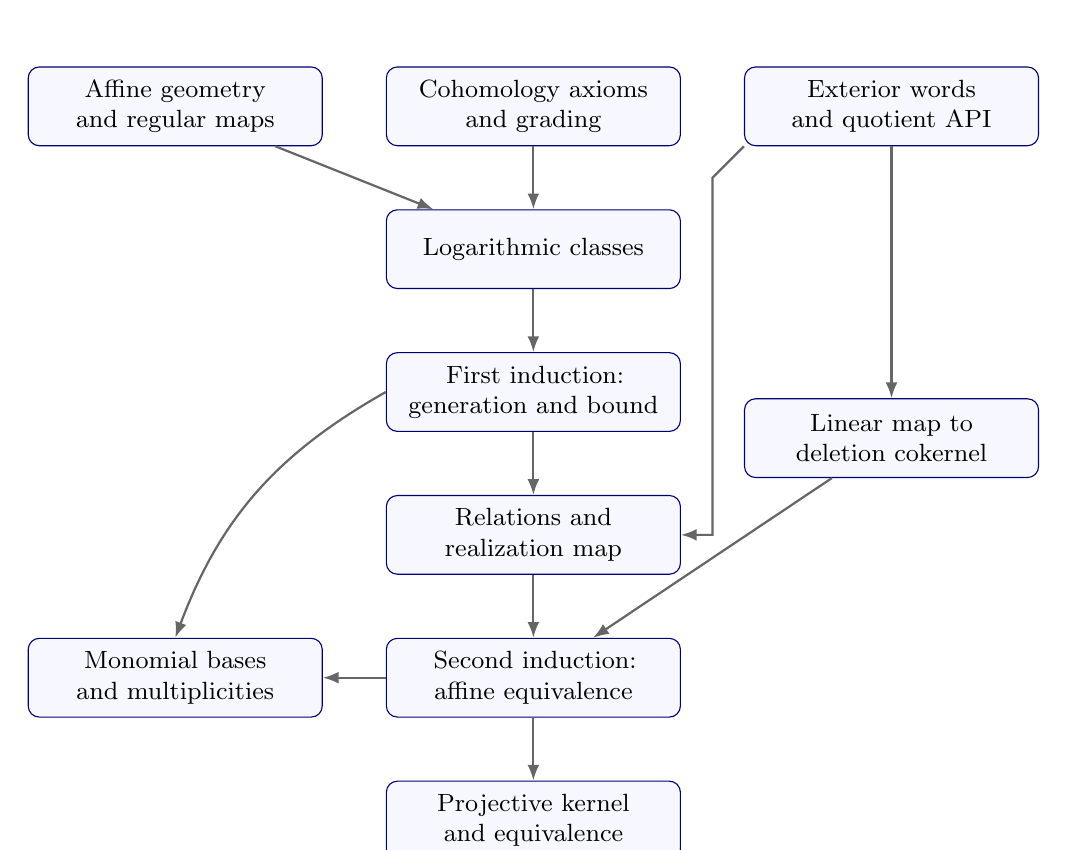
\begin{tikzpicture}[node distance=8mm and 8mm,
 box/.style={draw=blue!45!black,rounded corners,fill=blue!3,align=center,text width=35mm,minimum height=10mm,font=\small},
 arr/.style={-{Latex[length=2mm]},thick,draw=black!60}]
 \node[box] (geo) {Affine geometry\\and regular maps};
 \node[box,right=of geo] (ax) {Cohomology axioms\\and grading};
 \node[box,right=of ax] (alg) {Exterior words\\and quotient API};
 \node[box,below=of ax] (log) {Logarithmic classes};
 \node[box,below=of log] (ind1) {First induction:\\generation and bound};
 \node[box,below=of ind1] (rel) {Relations and\\realization map};
 \node[box,below=of alg,yshift=-24mm] (cok) {Linear map to\\deletion cokernel};
 \node[box,below=of rel] (iso) {Second induction:\\affine equivalence};
 \node[box,below=of iso] (proj) {Projective kernel\\and equivalence};
 \node[box,left=of iso] (basis) {Monomial bases\\and multiplicities};
 \draw[arr] (geo) -- (log);
 \draw[arr] (ax) -- (log);
 \draw[arr] (log) -- (ind1);
 \draw[arr] (ind1) -- (rel);
 \draw[arr] (alg) -- (cok);
 \draw[arr] (alg.south west) -- ++(-4mm,-4mm) |- (rel.east);
 \draw[arr] (rel) -- (iso);
 \draw[arr] (cok) -- (iso);
 \draw[arr] (iso) -- (proj);
 \draw[arr] (ind1.west) to[bend right=20] (basis.north);
 \draw[arr] (iso) -- (basis);
\end{tikzpicture}
\end{center}

The source annotations encode the full dependency graph, also supplied in \nolinkurl{dependencies.json}. The picture groups several nodes; it is not a replacement for that manifest. The stable extension branches directly from geometry, combinatorial recursion, and the stable realization interface.

\paragraph{Proposed module map.}
The following paths are planned Lean modules, not files claimed to compile in this bundle.
\begin{longtable}{@{}p{0.46\textwidth}p{0.49\textwidth}@{}}
\toprule
Module below \planned{ArrangementCohomology/} & Responsibility\\\midrule\endhead
\nolinkurl{Grading/Basic.lean} & Internal gradings, signs, homogeneous extraction.\\
\nolinkurl{Algebra/RelationQuotient.lean} & Two-sided relation submodule; algebra and linear descent.\\
\nolinkurl{Algebra/ExteriorWords.lean} & Word spanning, signs, boundary identities.\\
\nolinkurl{Algebra/Exact.lean} & Basis lifting and cokernel comparison.\\
\nolinkurl{Geometry/Arrangement.lean} & Hyperplanes, equations, intersections, restriction.\\
\nolinkurl{Geometry/Interface.lean} & Objects, maps, divisor pairs, commuting diagrams.\\
\nolinkurl{Geometry/Localization.lean} & Concrete coordinate-ring implementation of the interface.\\
\nolinkurl{Cohomology/Axioms.lean} & Ordinary theory and bridge from supports and purity.\\
\nolinkurl{Cohomology/Logarithms.lean} & The class on $\Gm$, logarithm identities, residues.\\
\nolinkurl{Cohomology/Deletion.lean} & First induction, short exactness, dimension, bases.\\
\nolinkurl{OrlikSolomon/Presentation.lean} & Definition, grading, base change, deletion map.\\
\nolinkurl{OrlikSolomon/Realization.lean} & Low-dimensional relation proof and realization map.\\
\nolinkurl{OrlikSolomon/Cokernel.lean} & The linear map $s$ and its surjectivity.\\
\nolinkurl{OrlikSolomon/Structure.lean} & Second induction and affine public theorem.\\
\nolinkurl{OrlikSolomon/Projective.lean} & Central boundary, kernel, deconing, projective theorem.\\
\nolinkurl{Combinatorics/Betti.lean} & Subset polynomials, counts, optional M\"obius formula.\\
\nolinkurl{Stable/Splitting.lean} & Abstract stable-category theorem.\\
\nolinkurl{Stable/Multiplicative.lean} & Optional sphere-graded evaluation and universal base change.\\
\nolinkurl{Examples/Sanity.lean} & Small arrangements and edge-case regressions.\\
\bottomrule
\end{longtable}

\paragraph{Public declaration shape.}
After bundling the interfaces and all necessary instances, the final declaration should have the following shape. Parameters displayed in square brackets here describe hypotheses or bundled structures; they are not a commitment to using typeclasses for every large datum.
\begin{lstlisting}
-- Design sketch only: names and notation require implementation.
noncomputable def affineEquiv
    [Field k] [CommRing R] [CommRing B] [Algebra R B]
    (G : ArrangementGeometry k)
    (H : OrdinaryTheory R B G)
    (A : AffineArrangement k V) :
    OrlikSolomon B A equiv_a[B] H.total (G.complement A)

theorem affineEquiv_homogeneous :
    PreservesBigrading (affineEquiv G H A)

theorem affineEquiv_generator (h : A.support) :
    affineEquiv G H A (generator h) =
      H.logClass (G.equationUnit A h)

noncomputable def projectiveEquiv
    (P : ProjectiveArrangement k W) (hne : P.Nonempty) :
    ProjectiveOrlikSolomon B P equiv_a[B]
      H.total (G.projectiveComplement P)
\end{lstlisting}

Use an ordinary \planned{AlgEquiv} plus a separate grading-preservation proof, rather than forcing the whole development through a new category of graded algebras at the outset. The first version can take $B=R[z,z^{-1}]$ to simplify coefficient plumbing, but the public general theorem should retain the weight-graded $B$ interface. This specialization is an implementation milestone, not a necessary mathematical assumption.

\paragraph{Milestone 1: reusable algebra and geometry contracts.}
Compile grading, exterior words, the relation quotient API, hyperplane equations, and the abstract geometry interface. Prove the componentwise/total exactness equivalence. Before any long proof, ensure one can form a module cokernel and descend a linear map through a two-sided relation quotient.

\paragraph{Milestone 2: logarithms and the first induction.}
Implement the ordinary theory, prove the $\Gm$ calculation and logarithm identities, then prove generation, the dimension bound, deletion short exactness, and the recursive basis theorem. The milestone theorem must not import the Orlik--Solomon structure theorem. This is the most useful early audit of the axioms.

\paragraph{Milestone 3: affine ring theorem.}
Implement the presentation, low-dimensional targets, relation checks, and realization map. Prove the representative identities and linear cokernel map, then apply the small comparison lemma in the second induction. Finish equation independence, grading, and coefficient base change.

\paragraph{Milestone 4: projective theorem and multiplicities.}
Implement the central signed boundary and its kernel, cone/decone geometry, and the projective equivalence. Add the subset-polynomial recurrence and basis counts. The M\"obius formula is optional for the first complete structure theorem.

\paragraph{Milestone 5: concrete adapters and generalized theories.}
Complete the coordinate-ring geometry adapter if it was developed separately. A geometry-conditional theorem is not yet the same deliverable as a theorem about actual algebraic arrangements. Separately implement the stable-category abstract deduction and, when available, concrete cohomology or stable realization instances.

\paragraph{Milestone 6: universal multiplication.}
For the widest multiplicative statement, formalize the sphere-graded symmetry and diagonal-cohomotopy coefficient algebra. Prove the canonical evaluation map respects multiplication, then use the stable splitting to prove it bijective as in Theorem~\ref{thm:universal-basechange}. This milestone depends on the stable branch, not on the ordinary point dimension axiom.

\section{Mathlib reuse, verification, and applications}

\paragraph{Verified library entry points.}
The online mathlib documentation was checked on 6 November 2026. It provides the following useful starting points; pin a Lean toolchain and mathlib revision before implementation, and verify exact signatures against that checkout. This blueprint does not claim to have tested a particular revision locally.
\begin{longtable}{@{}p{0.49\textwidth}p{0.46\textwidth}@{}}
\toprule
Existing entry point & Intended use\\\midrule\endhead
\nolinkurl{Mathlib.Algebra.Exact.Basic} & \planned{Function.Exact} and linear-map exactness facts.\\
\nolinkurl{Mathlib.LinearAlgebra.ExteriorAlgebra.Basic} & \planned{ExteriorAlgebra}, its generator map, and square-zero universal lift.\\
\nolinkurl{Mathlib.LinearAlgebra.ExteriorAlgebra.Basis} & Exterior bases and word spanning, where convenient.\\
\nolinkurl{Mathlib.LinearAlgebra.ExteriorAlgebra.Grading} & Existing exterior grading infrastructure.\\
\nolinkurl{Mathlib.Algebra.DirectSum.Decomposition} & Internal decomposition and homogeneous extraction.\\
\nolinkurl{Mathlib.Algebra.RingQuot} & Relation-generated noncommutative ring quotient and algebra lifts.\\
\nolinkurl{Mathlib.RingTheory.Ideal.Defs} & Ideals and two-sidedness infrastructure; inspect the chosen quotient API.\\
\bottomrule
\end{longtable}

Linear maps, submodules, module quotients, finite sums, finite-dimensional linear algebra, affine subspaces, multivariable polynomials, and localization provide the remaining basic infrastructure. The blueprint uses these established abstractions without promising that every needed convenience lemma already exists. In particular, the noncommutative quotient's \emph{linear} universal property and the graded antiderivation are explicit work items.

\paragraph{Required mathematical regression examples.}
These examples test errors in the statement or abstraction, not merely the syntax of implementation.
\begin{enumerate}
\item Empty affine arrangement in every dimension, including dimension zero: $C(U)=B$.
\item One hyperplane: exterior algebra on one generator. Its square is zero with coefficients in $\Z/2$ and $\Z/4$.
\item The $n$ coordinate hyperplanes: the full exterior algebra and $P(t)=(1+t)^n$.
\item Two parallel affine lines: $e_1e_2=0$, but $e_2-e_1\ne0$ over a nonzero coefficient ring; $P(t)=1+2t$.
\item Three distinct concurrent lines: $e_2e_3-e_1e_3+e_1e_2=0$ and $P(t)=1+3t+2t^2$. Restriction has duplicate intersections that must be discarded.
\item Three nonconcurrent affine lines with no parallel pair: the triple intersection is empty, so $e_1e_2e_3=0$ and $P(t)=1+3t+3t^2$. There is no degree-two boundary relation for that triple.
\item The two rational points in $\A^1_{\mathbf F_2}$: the complement has no $\mathbf F_2$-points, but its coordinate localization is nonzero and its polynomial is $1+2t$.
\item One projective hyperplane: affine-space cohomology. For $m\geq1$ distinct points in $\PP^1$, the polynomial is $1+(m-1)t$.
\item Zero coefficient ring: the equivalence still makes sense; do not infer a unique basis cardinal from a zero module.
\end{enumerate}

\paragraph{Completion criteria.}
Every planned declaration attached to a definition, lemma, or theorem should exist and compile. All public theorem dependencies must be free of \planned{sorryAx}; inspect actual axiom reports, not just a text search for \planned{sorry}. Verify that the cohomology structure has precisely the standard inputs listed above, and that the concrete geometry adapter is proved if the public theorem is stated for actual schemes. Run \planned{lake build} and declaration-link checks after fixing the package versions. Then mark verified statements and proofs in the blueprint. Until that happens, the annotations are proposed declaration links only.

\paragraph{Concrete cohomology instances.}
Geometric Betti and geometric \(\ell\)-adic cohomology with the usual integral, torsion, or field coefficients are intended ordinary instances; in the latter case $\ell$ is invertible in the base field. Characteristic-zero algebraic de Rham and rigid cohomology are further intended examples. Standard localization and purity theorems must be supplied when building each instance. Ordinary crystalline cohomology of a nonproper smooth variety is not automatically an instance: the needed affine-line invariance fails in the naive theory. Rational log-crystalline or overconvergent replacements require their own precise setup. These are application boundaries, not extra hypotheses silently added to the formal theorem.

Naturality can retain Galois or Frobenius actions by adding actions on the graded modules that commute with pullback, product, and residue. The canonical logarithmic map is then equivariant by uniqueness of $\tau$ and naturality. This is an extension of the interface; it does not require redoing the induction. For a split arrangement, the geometric diagonal generators are fixed under the relevant action, with the Tate action retained in $B_w$.

\paragraph{What this bundle has verified.}
The document builds as a PDF. The dependency manifest is extracted from the source, every dependency resolves to a node, and the resulting directed graph is acyclic. This is a consistency check on the blueprint, not a formal verification of the mathematics. No Lean executable was available in the authoring environment, so the displayed signatures and planned declarations have not been elaborated or kernel-checked. The bundle intentionally contains no purported proof files filled with unproved placeholders.

\section{Sources and further context}

The mathematical proofs in the core blueprint are supplied above, rather than delegated to a comparison theorem. The following sources provide the broader context and the verified software interfaces.
\begin{enumerate}
\item P. Orlik and L. Solomon, \emph{Combinatorics and topology of complements of hyperplanes}, Inventiones Mathematicae 56 (1980), 167--189. The classical algebra presentation.
\item A. Chatzistamatiou, \emph{Motivic cohomology of the complement of hyperplane arrangements}, \url{https://arxiv.org/abs/math/0601737}. Motivic splitting and arithmetic coefficient phenomena.
\item D.-C. Cisinski and F. D\'eglise, \emph{Mixed Weil cohomologies}, \url{https://arxiv.org/abs/0712.3291}. A standard sufficient cohomology formalism.
\item K. Peng, \emph{Milnor--Witt motivic cohomology of complements of hyperplane arrangements}, \url{https://arxiv.org/abs/2005.12139}. The distinction between ordinary exterior relations and the quadratic refinement.
\item F. Morel, \emph{The stable $\A^1$-connectivity theorems}, K-Theory 35 (2005), 1--68. Connectivity input for the stable extension.
\item Mathlib documentation: \url{https://leanprover-community.github.io/mathlib4_docs/Mathlib/Algebra/Exact/Basic.html}; \url{https://leanprover-community.github.io/mathlib4_docs/Mathlib/LinearAlgebra/ExteriorAlgebra/Basic.html}; \url{https://leanprover-community.github.io/mathlib4_docs/Mathlib/Algebra/DirectSum/Decomposition.html}; \url{https://leanprover-community.github.io/mathlib4_docs/Mathlib/Algebra/RingQuot.html}.
\item Patrick Massot and contributors, \emph{leanblueprint}, \url{https://github.com/PatrickMassot/leanblueprint}. The source uses its standard declaration and dependency annotations. A web build and declaration checks require the corresponding tooling and a Lean project; the supplied standalone PDF build does not.
\end{enumerate}

\end{document}
